% Fair topics for CS340 MIDTERM:
% \begin{enumerate}
%     \item test vs. training
%     \item decision trees
%     \item decision stumps
%     \item naive Bayes
%     \item k-nn
%     \item ensemble methods
%     \item clustering
%     \item outlier detection
%     \item least squares
%     \item norms
%     \item change of bases (polynomial bases)
%     \item log-sum-exp
%     \item huber
%     \item gradient descent
%     \item linear 
%     \item nearest neighbors
%     \item k-means clustering
%     \item naive Bayes
%     \item Probabilistic classification
%     \item cross validation
% \end{enumerate}

\documentclass{article}

\usepackage{fullpage}
\usepackage{color}
\usepackage{amsmath}
\usepackage{url}
\usepackage{verbatim}
\usepackage{graphicx}
\usepackage{subcaption}
\usepackage{parskip}
\usepackage{amssymb}
\usepackage{amsfonts}
\usepackage{nicefrac}
\usepackage{listings} % For displaying code
\usepackage{algorithm2e} % pseudo-code
\usepackage{natbib}
\usepackage{todonotes}

% Answers
\def\rubric#1{\gre{Rubric: \{#1\}}}{}

% Colors
\definecolor{blu}{rgb}{0,0,1}
\def\blu#1{{\color{blu}#1}}
\definecolor{gre}{rgb}{0,.5,0}
\def\gre#1{{\color{gre}#1}}
\definecolor{red}{rgb}{1,0,0}
\def\red#1{{\color{red}#1}}
\def\norm#1{\|#1\|}

% Math
\def\R{\mathbb{R}}
\def\argmax{\mathop{\rm arg\,max}}
\def\argmin{\mathop{\rm arg\,min}}
\newcommand{\mat}[1]{\begin{bmatrix}#1\end{bmatrix}}
\newcommand{\alignStar}[1]{\begin{align*}#1\end{align*}}
\def\half{\frac 1 2}

% LaTeX
\newcommand{\fig}[2]{\includegraphics[width=#1\textwidth]{#2}}
\newcommand{\centerfig}[2]{\begin{center}\includegraphics[width=#1\textwidth]{#2}\end{center}}
\def\items#1{\begin{itemize}#1\end{itemize}}
\def\enum#1{\begin{enumerate}#1\end{enumerate}}

% My stuff
\def\ans#1{\par\gre{Answer: #1}}
\definecolor{codegreen}{rgb}{0,0.6,0}
\definecolor{codegray}{rgb}{0.5,0.5,0.5}
\definecolor{codepurple}{rgb}{0.58,0,0.82}
\definecolor{backcolour}{rgb}{0.95,0.95,0.92}

\lstdefinestyle{mystyle}{
    backgroundcolor=\color{backcolour},   
    commentstyle=\color{codegreen},
    keywordstyle=\color{magenta},
    numberstyle=\tiny\color{codegray},
    stringstyle=\color{codepurple},
    basicstyle=\ttfamily\footnotesize,
    breakatwhitespace=false,         
    breaklines=true,                 
    captionpos=b,                    
    keepspaces=true,                 
    numbers=left,                    
    numbersep=5pt,                  
    showspaces=false,                
    showstringspaces=false,
    showtabs=false,                  
    tabsize=1
}
\lstset{style=mystyle}

\begin{document}

% \begin{enumerate}
% \item Classifier 1\\
% \item Classifier 2\\
% \item Classifier 3\\
% \item Meta Classifier\\
% \end{enumerate}



\setcounter{section}{0}

\section{Team}
\begin{tabular}{|c | c |} 
\hline
Team Members & CS id: d8z9a Student id: 53033149 \\
\hline
Kaggle Team Name & onlyme \\
\hline
\end{tabular}
\section{Solution Summary}

The solution uses features cases, cases\_14\_100k, cases\_100k, deaths to predict the death count of the next days. In this model, we fit a linear regression of the features, and the next prediction is done with the predictions of the next feature itself. Also the following model has hyper-parameters $k$ (number of time-series to look behind), $p$ (the polynomial basis), $log\_base$ (to use log base or not) and $use\_prediction$ (to use the predicted death value for the next prediction or the prediction from the feature itself).\\~\\
The best solution to get is the hyper-parameters that minimizes the error function. The best hyper-parameters are chosen by training the data to the date given by phase1 and predict the next days.
\section{Experiments}

\subsection*{Feature Selection}

The following are chosen as features: cases, cases\_100k, cases\_14\_100k and deaths to predict the next death cases for next day. The deaths will also be input in our feature selection because it modifies the value for the next death number cases.

Below are some plots related to our features.

\begin{figure}[h]
    \centering
    \begin{subfigure}[b]{0.24\linewidth}
        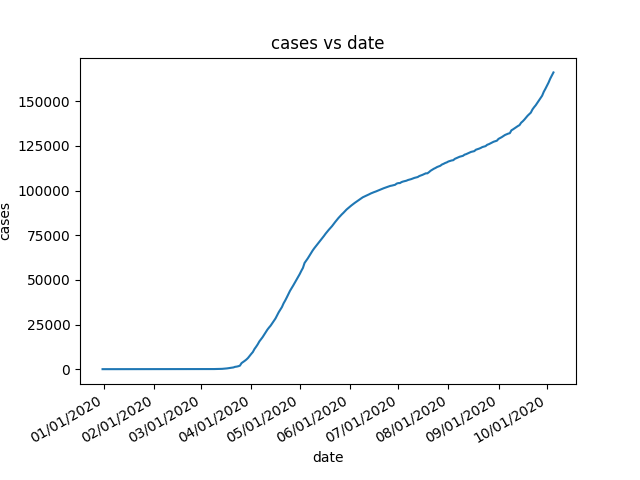
\includegraphics[width=\linewidth]{../figs/cases.png}
        \caption{cases}
    \end{subfigure}
    \begin{subfigure}[b]{0.24\linewidth}
        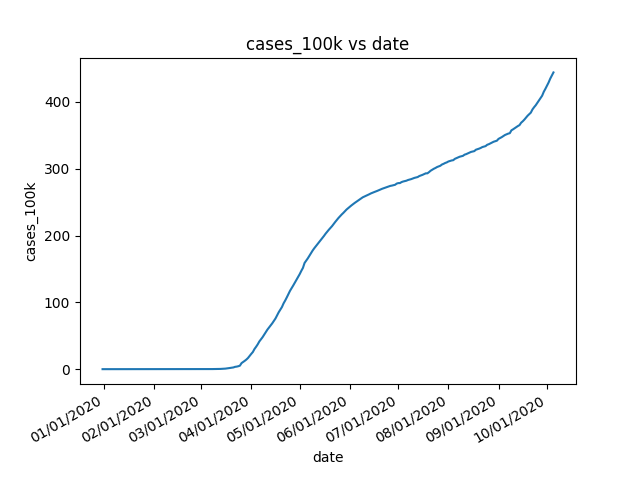
\includegraphics[width=\linewidth]{../figs/cases_100k.png}
        \caption{cases\_100k}
    \end{subfigure}
    \begin{subfigure}[b]{0.24\linewidth}
        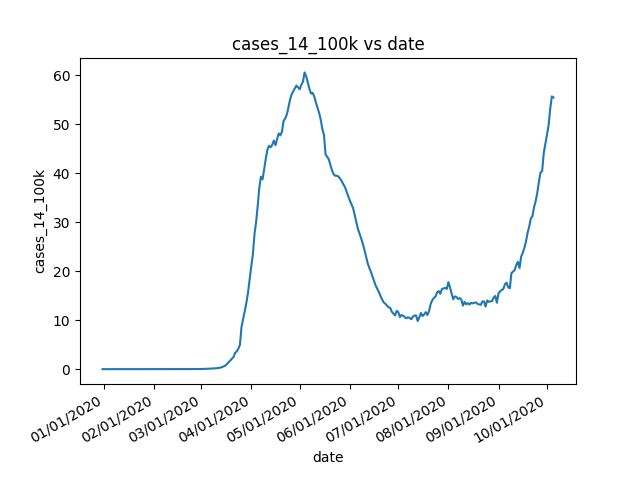
\includegraphics[width=\linewidth]{../figs/cases_14_100k.png}
        \caption{cases\_14\_100k}
    \end{subfigure}
    \begin{subfigure}[b]{0.24\linewidth}
        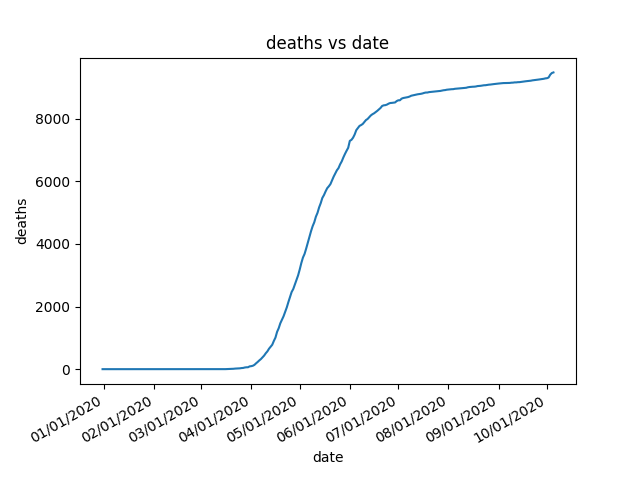
\includegraphics[width=\linewidth]{../figs/deaths.png}
        \caption{deaths}
    \end{subfigure}
    \caption{Plots of cases vs date}
\end{figure}

\begin{figure}[h]
    \centering
    \begin{subfigure}[b]{0.24\linewidth}
        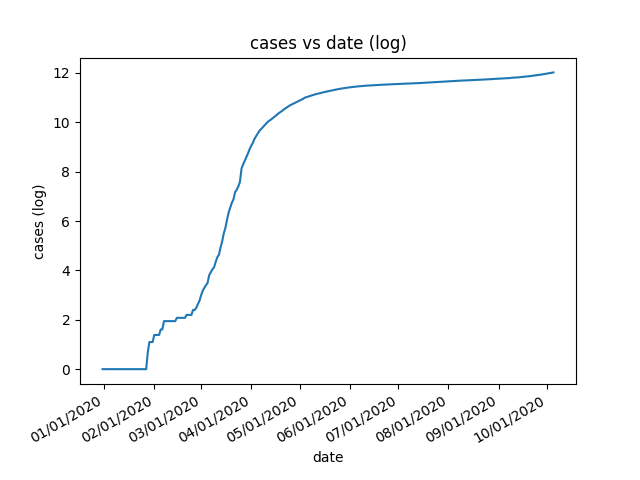
\includegraphics[width=\linewidth]{../figs/cases_log.png}
        \caption{cases (log)}
    \end{subfigure}
    \begin{subfigure}[b]{0.24\linewidth}
        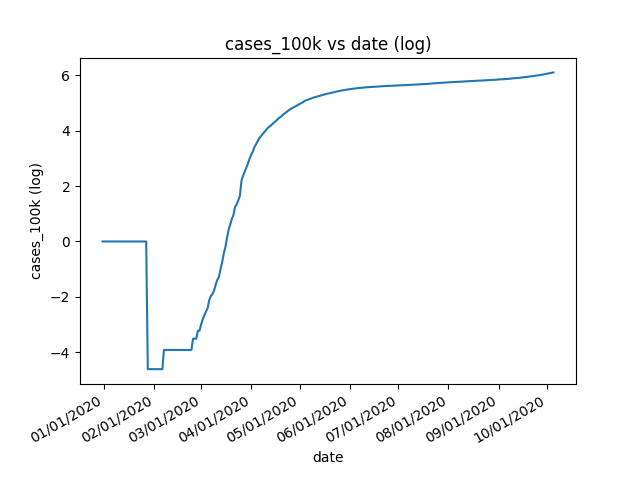
\includegraphics[width=\linewidth]{../figs/cases_100k_log.png}
        \caption{cases\_100k (log)}
    \end{subfigure}
    \begin{subfigure}[b]{0.24\linewidth}
        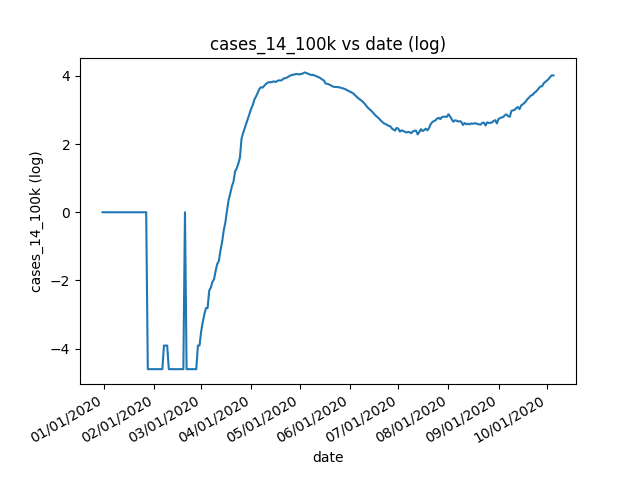
\includegraphics[width=\linewidth]{../figs/cases_14_100k_log.png}
        \caption{cases\_14\_100k (log)}
    \end{subfigure}
    \begin{subfigure}[b]{0.24\linewidth}
        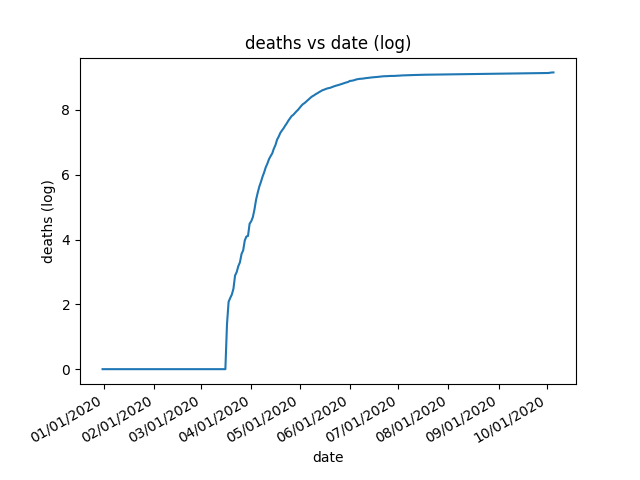
\includegraphics[width=\linewidth]{../figs/deaths_log.png}
        \caption{deaths (log)}
    \end{subfigure}
    \caption{Plots of cases\_100k vs date}
\end{figure}

The log base models are trained as well since we may be dealing with big numbers that polynomial basis cannot handle well. Also since it is a prediction with the case of a virus, we know a graph more or less has to be right skewed. 

\subsection*{Hyperparameters}

\textbf{Choosing $k$ hyperparameter}

The $k$ hyperparameter can be anything that is greater than 0 and less than the size of the feature. We chose this $k$ value by trying bunch of different values for $k$. In general $k$ can be anything that best fits our model.

\textbf{Choosing $p$ hyperparameter}

In general, based on the graphs defined in Figure 1, we can see that no more than $p > 5$ is needed. Also since a greater number of $p$ greatly influences the edges of our model (which is bad for predicting the future) having a big $p$ will lead to extreme numbers as each time we try to predict the next values. Hence our hyperparameter will be $p < 5$ in general cases.

The value of $p$ will also be affected greatly by the $k$ hyperparameter. A big $k$ will look at the $k$ past data, so the greater $k$ is, a greater $p$ might generate a better fit while the lower $k$ is, a linear fit might be better.

\textbf{Other hyperparameters}

The $log\_base$ and $use\_prediction$ are just binary inputs to whether we would like to use a log based data set to generate the model or use the prediction based on the fit of all data, or just keep using the fit from the death feature column.

\subsection*{Training}

Training is done via minimizing our error function depending on our values of hyperparameters. For different values of $k$, $p$, $log\_base$, $use\_prediction$, we try to get the best values that minimizes the error.

\textbf{Phase 1}

In general for phase 1, the hyper parameters are chosen by fitting a model based on features until October 5 and then trying to minimize the error by comparing with next 11 days (October 16).

Below is a table summarizing the trials.

\begin{center}
    \begin{tabular}{|c | c | c | c | c |} 
    \hline
    $log\_base$ & $use\_prediction$ & $k$ & $p$ & $min(\sum (y_{pred} - y)^2)$  \\ [0.5ex]
    \hline\hline
    False & False & 88  & 1 & 1177.149 \\
    \hline
    False & True  & 127 & 1 & 1313.394 \\
    \hline
    True  & False & 81  & 1 & 1678.265 \\
    \hline
    True  & True  & 137 & 2 & 1372.992 \\
    \hline
   \end{tabular}\\~\\
   Table 1: Table summarizing $k$ and $p$ results for different $log\_base$ and $use\_prediction$ (phase 1)
\end{center}

For phase 1, the minimum error is given when $log\_base = False$, $use\_prediction = False$, $k = 88$, $p = 1$.

\textbf{Phase 2}

For phase 2, the values for the hyperparameters are also found using the same strategy for phase 1, now except trying to get best result from next 11 days starting October 5, the test is done with the next 20 days starting on October 5.

Below is the table summarizing the trials.

\begin{center}
    \begin{tabular}{|c | c | c | c | c |} 
    \hline
    $log\_base$ & $use\_prediction$ & $k$ & $p$ & $min(\sum (y_{pred} - y)^2)$  \\ [0.5ex]
    \hline\hline
    False & False & 88  & 1 & 2184.482 \\
    \hline
    False & True  & 127 & 1 & 3198.579 \\
    \hline
    True  & False & 81  & 1 & 2210.375 \\
    \hline
    True  & True  & 79  & 1 & 1954.314 \\
    \hline
   \end{tabular}\\~\\
   Table 2: Table summarizing $k$ and $p$ results for different $log\_base$ and $use\_prediction$ (phase 2)
\end{center}

The only difference between Table 1 and Table 2 is the last row. Phase 1's $k = 137$ and $p = 2$ could not possibly be used for further predictions because of the polynomial extreme values going faster over each prediction. Hence we got a new value $k = 79$ and $p = 1$ which we will use it to predict the next 5 days using now all data until October 25.

\section{Results}

\begin{center}
 \begin{tabular}{|c | c | c |} 
 \hline
 Team Name & Kaggle Phase 1 Score & Kaggle Phase 2 Score  \\ [0.5ex]
 \hline\hline
onlyme & 10.13544 & N/A  \\
 \hline
\end{tabular}
\end{center}

\section{Code}


\begin{lstlisting}[language=Python, caption=AutoRegressor class implementation]
class AutoRegressor:
    def __init__(self, k, p=1, 
                log_base=False,
                use_prediction=True,
                model=LeastSquares):
        """
        k                   = the number of data sets to look behind to make next prediction
        p                   = polynomial basis
        log_base            = change data to log space
        use_prediction      = use prediction from X_k to test y_k+1, if false uses
                              time series the the deaths column itself
        model               = the linear model to use. We only use Least Squares
        In this class, everything with variable X means it is not weighted
        everything with variable Z means it has been transformed/weighted.
        """
        self.k = k
        self.p = p
        self.log_base = log_base
        self.use_prediction = use_prediction
        self.model = model
        self.y_model = model()

    def fit(self, X, y):
        N,D = X.shape
        k = self.k

        # if k is too large don't do this.
        self.size = N - k
        if (self.size <= 0): return

        # transform X to Z using transform method.
        Z = self.__transform(X)
        # get values of y for time series
        y_k = y[self.size:N]

        # set our features to predict next features.
        self.__feature_time_series(X, Z)
        # our general prediction for y_k+1
        self.y_model.fit(Z, y_k)

    def __feature_time_series(self, X, Z):
        """
        Grabs data from k to N-1 for each feature. If p > 0, also adds polynomial basis
        columns.
        Generates models to predict x_i_k+1 so that we can comput y_k+1.
        The models here are by independent, meaning they will have their own
        bias when fitting and predicting the model.
        """
        N, D = X.shape
        p = self.p

        feature_models = []
        for i in range(D):
            pos = i*p+1
            # grab the data from Z and add a bias 1 or e.
            x_i = self.__add_bias(Z[:,pos:pos+p])
            x_k = X[self.size:N,i]
            # create model and fit.
            model = self.model()
            model.fit(x_i, x_k)
            # save model to predict x_i_k+1
            feature_models.append(model)

        self.feature_models = feature_models

    def __transform(self, X):
        """
        Transforms X into Z. Adds the bias 1 if non logbase, e if logbase.
        Adds polynomial basis given p.
        """
        N,D = X.shape
        k = self.k
        p = self.p

        # new data set
        Z = np.ones(shape=(k, D*p+1))
        k_data = X[self.size-1:N-1, :]

        for i in range(D):
            pos = i*p+1
            # add polynomial basis
            Z[:,pos:pos+p] = self.__polyBasis(k_data[:,i])

        # handle log case
        if self.log_base == True:
            Z[:,0] = np.exp(1)

        return Z

    def __polyBasis(self, X):
        """
        General function to change to poly basis.
        NOTE: this does not add 1 as a bias.
        """
        N = X.size
        p = self.p

        Z = np.ones((N, p))
        for j in range(1, p + 1):
            Z[:,j-1] = X**j

        return Z

    def __add_bias(self, X):
        """
        Adds a bias of e if log_base, 1 otherwise.
        """
        N,D = X.shape
        Z = np.ones(shape=(N,D+1))
        Z[:,1:] = X

        if self.log_base == True:
            Z[:,0] = np.exp(1)

        return Z

    def predict(self, X, num_times):
        """
        Predict the next sequence of num_times.
        """
        def append_time_series(Z, y_k):
            """
            Predict x_i_k+1, removes x_i_1 from Z, and appends the new value.
            If use_prediction is on, it will use the predicted value y_k+1 and its 
            polynomial biases for next predict. Else it will use the values from
            its features series x_i_k+1.
            """
            N,D = Z.shape
            p = self.p
            feature_models = self.feature_models

            i = 0
            time_preds = np.ones(shape=(1,D))
            for model in feature_models:
                # predict the new features
                pos = i*p+1
                x_i = self.__add_bias(Z[:,pos:pos+p])
                pred = model.predict(x_i)[-1]
                i += 1

                time_preds[:,pos:pos+p] = self.__polyBasis(pred)

            # determine log base
            if self.log_base == True:
                time_preds[:,0] = np.exp(1)

            # remove first row, append to last row.
            Z = Z[1:]
            Z = np.append(Z, time_preds, axis=0)

            # use prediction will change the deaths column to predicted value and its
            # polynomial basis.
            if self.use_prediction == True:
                Z[:,pos:pos+p] = self.__polyBasis(y_k)

            return Z

        Z = self.__transform(X)
        y_k = self.y_model.predict(Z)[-1]
        
        y_pred = np.zeros(num_times)

        for i in range(num_times):
            # predict, and save results.
            Z = append_time_series(Z, y_k)
            y_k = self.y_model.predict(Z)[-1]
            y_pred[i] = y_k

        return y_pred
\end{lstlisting}

\begin{lstlisting}[language=Python, caption=Main function]
if __name__ == "__main__":
    # modify variables here
    phase = "phase2"        # the phase to test
    num_data = 5            # the number of data to predict
    log_base = True         # variable if our model is in log base or not
    use_prediction = True   # variable to use predictions in general over time series

    # load file + set data
    df = pd.read_csv(os.path.join("..", "data", phase + "_training_data.csv"))
    
    X_codes = df.country_id.unique()
    X_codes = X_codes[X_codes != "CA"]

    X_ca = df.loc[df["country_id"] == "CA"]

    ca_cases = X_ca["cases"].values
    ca_100k = X_ca["cases_100k"].values
    ca_14_100k = X_ca["cases_14_100k"].values
    ca_deaths = X_ca["deaths"].values
    dates = X_ca["date"].values

    # combine column
    X = np.column_stack((ca_cases, ca_100k, ca_14_100k, ca_deaths))

    # if we are using log space
    if log_base == True:
        X = np.log(X)
        X[X == -np.inf] = 0

        ca_deaths = np.log(ca_deaths)
        ca_deaths[ca_deaths == -np.inf] = 0

    # run test only in phase 1 mode
    # this only works phase 1 data.
    # uncomment next line to get best k and p. NOTE: num_data has to be either 11 or 20
    # __find_min_poly_basis(X, ca_deaths, num_data, log_base, use_prediction)
    
    # code for plots
    # dates_obj = [dt.datetime.strptime(d, "%m/%d/%Y").date() for d in dates]
    # labels = ["cases vs date", "cases_100k vs date", "cases_14_100k vs date", "deaths vs date"]
    # ylabels= ["cases", "cases_100k", "cases_14_100k", "deaths"]
    # fnames = ["cases", "cases_100k", "cases_14_100k", "deaths"]

    # for i in range (4):
    #     if log_base == True:
    #         __plot(dates_obj, X[:,i], fnames[i]+"_log", labels[i] + " (log)", "date", ylabels[i] + " (log)")
    #     else:
    #         __plot(dates_obj, X[:,i], fnames[i], labels[i], "date", ylabels[i])
        

    # fit to autogressor model
    model = AutoRegressor(k=79, p=1, log_base=log_base, use_prediction=use_prediction)
    model.fit(X, ca_deaths)
    y_preds = model.predict(X, num_data)

    if log_base == True:
        y_preds = np.exp(y_preds)

    y_preds = y_preds.astype('int64')
    print(y_preds)
    
    # to csv
    output = pd.DataFrame({'deaths': y_preds,
                           'id': range(num_data)})
    out_path = os.path.join("..", "data", phase + "_out.csv")
    output.to_csv(path_or_buf=out_path,index=False)
\end{lstlisting}
\clearpage
\begin{lstlisting}[language=Python, caption=Brute force to search for k and p]
def __find_min_poly_basis(X, y, num_data, log_base=False, use_prediction=True):
    # first is for predicting 11 days in the future
    # second is for predicting 20 days in the future
    # comment/uncomment as needed 
    # y_test = [9504,9530,9541,9557,9585,9585,9585,9627,9654,9664,9699]
    y_test = [9504,9530,9541,9557,9585,9585,9585,9627,9654,9664,9699,
              9722,9746,9760,9778,9794,9829,9862,9888,9922]

    min_error = np.inf

    for p in range(1,5):
        for k in range(1, 280):
            model = AutoRegressor(k=k, p=p, log_base=log_base, use_prediction=use_prediction)
            try:
                model.fit(X, y)
            except:
                continue
            y_preds = model.predict(X, num_data)
            if log_base == True:
                y_preds = np.exp(y_preds)
            error = np.sum(np.square(y_preds-y_test))
            # print("p: %d, k: %d, error: %.3f" % (p, k, error))
            if (error < min_error):
                p_low = p
                k_low = k
                min_error = error
    
    print("lowest p: %d, k: %d, error: %.3f" % (p_low, k_low, min_error)) 
\end{lstlisting}

\begin{lstlisting}[language=Python, caption=Plotting function]
def __plot(x, y, fname, label, xlabel, ylabel):
    plt.gca().xaxis.set_major_formatter(mdates.DateFormatter('%m/%d/%Y'))
    plt.gca().xaxis.set_major_locator(mdates.MonthLocator())
    plt.plot(x, y)
    plt.gcf().autofmt_xdate()
    plt.title(label)
    plt.xlabel(xlabel)
    plt.ylabel(ylabel)
    plt.savefig(os.path.join("..", "figs", fname))
    plt.clf()
\end{lstlisting}

\section{Conclusion}
In this project, I have learned how to do auto regressive models in general. I learned how to implement and interpret them. I have learned the importance of how to look at a data and transform it into a model. This was the hardest part of the project since we had to start barebone with just brief hints. Finally, I learned that when fitting a model, one should go from a simple model to complex, since trying to make something complex may not work well, which I ended up wasting a lot of time.

If I were given more time, I would have tried to get nearest neighbors of canada using KNN and also add them to the feature space. Also I would have tried doing multiple transformations into on feature space. For example, right now the model I implemented it either uses all polynomial basis of 3, or all basis of 2. I could have mixed this up for each feature, having different polynomial basis depending on the model which I would do the same case for the log space. Finally I would try using more linear transformations instead of just polynomial.

\section{Additional Notes}

Code style from: \url{https://www.overleaf.com/learn/latex/code_listing}

\newpage




\end{document}
